\chapter{Communication Technologies}\label{Communications}

% Add Social Media?

\newenvironment{ucclist}[1]
{
	\begin{mdframed}
	\subsection{#1}
	\begin{mdframed}
		Address:  <\href{mailto:#1@ucc.asn.au}{#1@ucc.asn.au}>
	\end{mdframed}
	\begin{mdframed}
		Subscribe:  \url{http://lists.ucc.asn.au/mailman/listinfo/#1}
	\end{mdframed}


	
}{\end{mdframed}}

\section{Mailing Lists}

\textsc{TO THE LISTS!}
\begin{ucclist}{ucc-announce}

An announcement list through which we let 
members know about Events and the like. You are automatically 
subscribed to this list when becoming a member. 

\end{ucclist}

\begin{ucclist}{ucc}

Having a party that you want to invite UCCans to? This is the 
list for you! Most UCCans subscribe to this list so it's a great 
source of information and discussion on both the club and general 
technical things. 

\end{ucclist}

\begin{ucclist}{committee}
The list where committee matters are dealt with and circular 
discussions occur. If you are interested in the running of the club then 
you should subscribe to this list. 
\end{ucclist}

\begin{ucclist}{tech}
Technical question? Suggestions or discussion around UCCs setup? 
The list used to discuss UCC's hardware and machines. 
\end{ucclist}

\pagebreak
\section{IRC}


\begin{mdframed}
Without a doubt, the easiest way to waste time in or out of UCC 
is chatting on our Internet Relay Chat (IRC) server. 

You'll get to chat with some of the older members of the club who 
may not even be in Perth. Some of these old guard may seem a 
little grumpy or intimidating at first, but give them a chance, they 
are gold mines for information about the club and all things tech! 
We also have members from CASSA and ComSSA, clubs at other WA unis. 

You can connect with an IRC client to \texttt{irc://irc.ucc.asn.au:6667} 
and join the channel \texttt{\#ucc}, or with a web browser go to 
\url{http://irc.ucc.asn.au}

\begin{figure}[H]
	\centering
	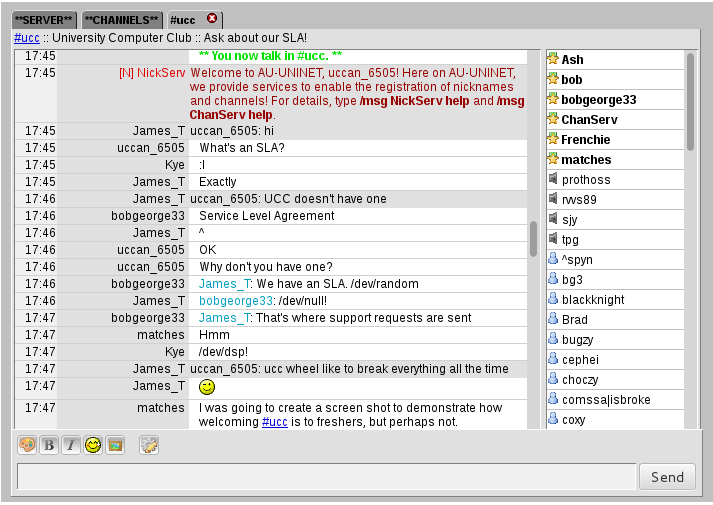
\includegraphics[width=0.8\textwidth]{figures/webirc.png}
	\caption{What normally happens when a Fresher joins IRC}
	\label{webirc.jpg}
\end{figure}

IRC produces some incredible quotes. You can see these at \url{http://zanchey.ucc.asn.au/qdb/}.

I didn't say they were wise or funny, just incredible.

\end{mdframed}

\section{Social Media}

\begin{mdframed}

Dragging itself kicking and screaming into the 21st Century, UCC has managed to set up a social media presence in something called the "cloud".

\begin{itemize}
\item The UCC Facebook Group is located at: 

\url{https://www.facebook.com/groups/universitycomputerclub/}
\item The UCC Status Twitter Account (used mainly to tell everyone things are broken): \url{https://twitter.com/ucc_status}
\item GitHub: \url{https://github.com/ucc}

\end{itemize}

\end{mdframed}
